%\textit{Describe experiments: we will design benchmarks per model
%Describe alternative algorithms }
%a) \textit{single-arm solution per model,}
%b) \textit{exhaustive search integrated with the corresponding path planner for each model,}
%c) \textit{approximate solution we propose [unless we come up with something
%  better for the easier models].}
%d) \textit{1-TSP broken into 2 and coordinated}
%
%\textit{What do we measure: a) solution quality in terms of the cost metrics
%identified and b) computation time.}

\begin{figure}[h]
\vspace{-0.1in}
	\centering
		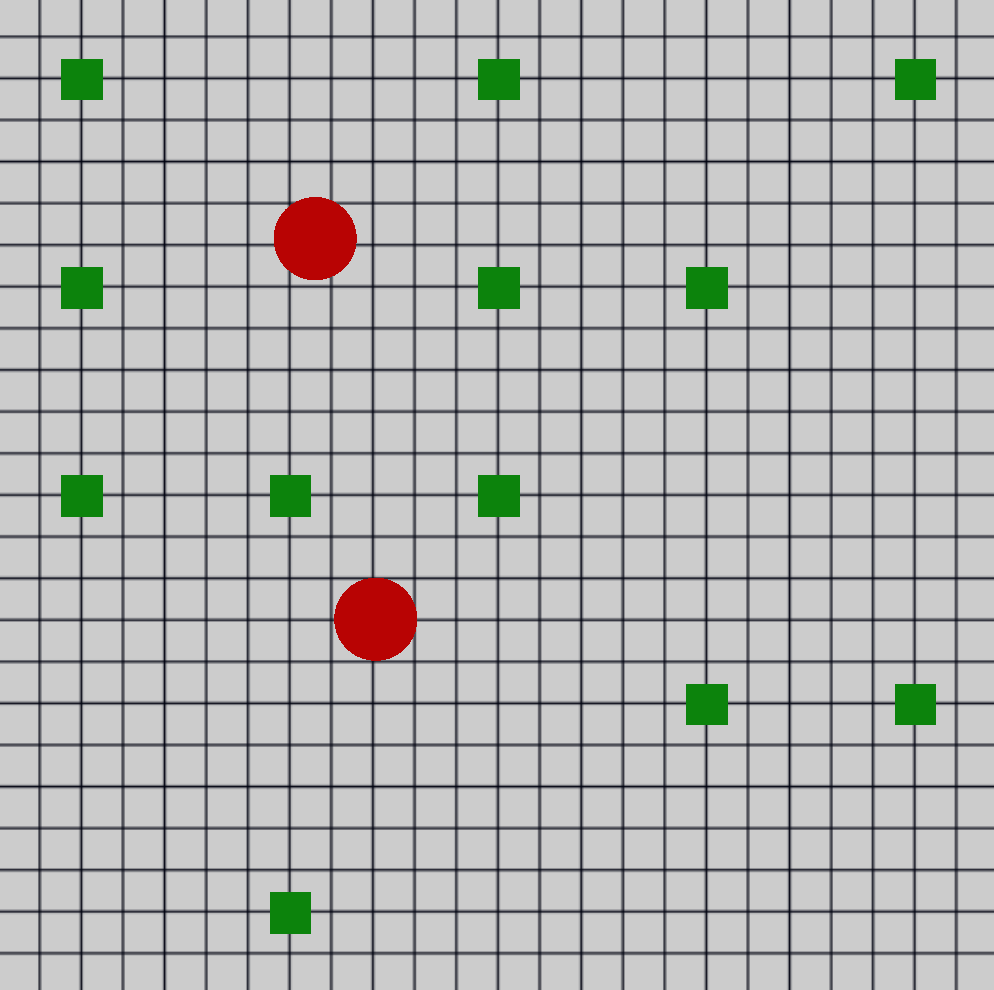
\includegraphics[width=0.245\textwidth,trim={1cm 9cm 1cm 5cm},clip]{figures/simple_picker_benchmark}
		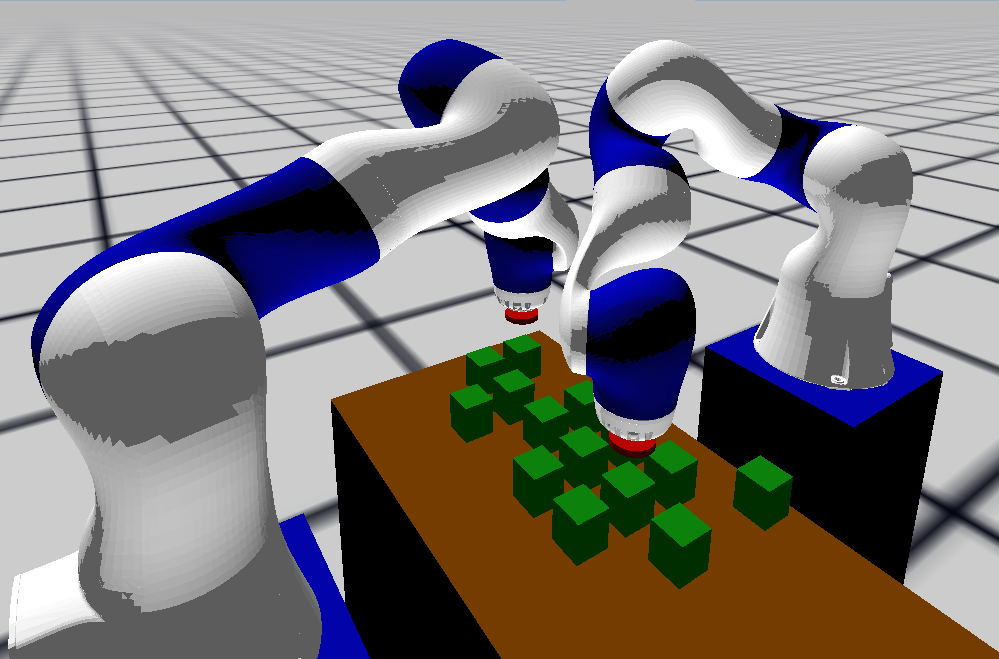
\includegraphics[width=0.235\textwidth]{figures/kuka_benchmark2}
%		\vspace{-.3in}
		\caption{\textit{Picker} and \textit{Manipulator} trials.}
		\label{fig:benchmarks}
\vspace{-0.1in}
\end{figure}


\begin{figure*}[t]
%\vspace{-0.2in}
	\centering
%	\includegraphics[width=2.1in]{figures/disk_solution}
%	\includegraphics[width=2.1in]{figures/disk_timing}
%	\includegraphics[width=2.1in]{figures/disk_more_solution}
%	\includegraphics[width=2.1in]{figures/disk_more_timing}

%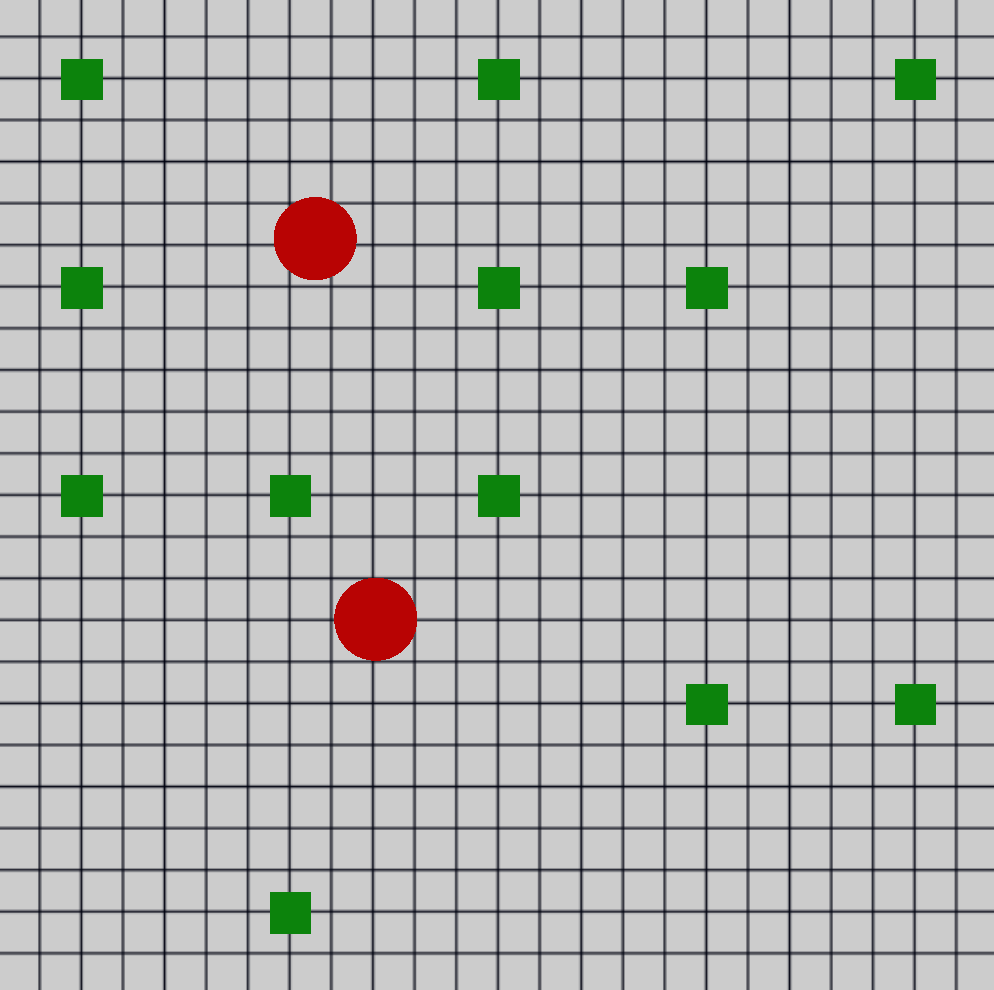
\includegraphics[width=0.48\textwidth,trim={1cm 9cm 1cm 5cm},clip]{figures/simple_picker_benchmark}\\
	
\includegraphics[width=0.6\textwidth]{figures/results/labels}
	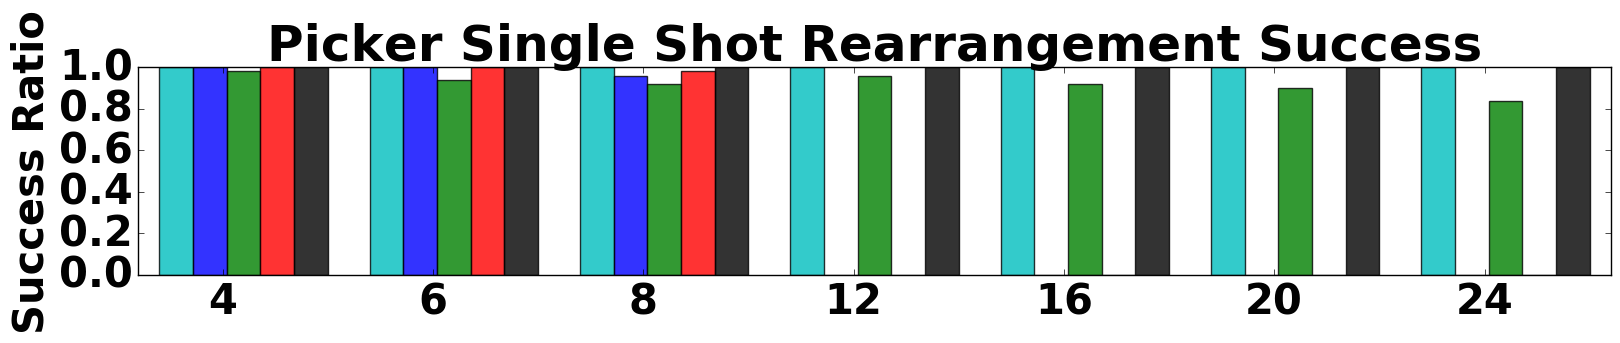
\includegraphics[width=0.48\textwidth]{figures/results/4_sp_ms_success}
	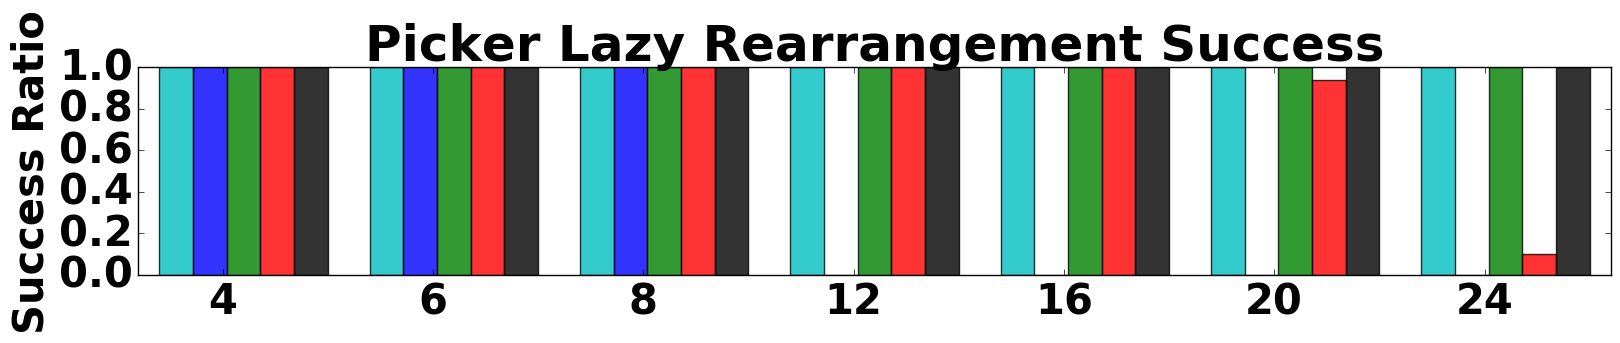
\includegraphics[width=0.48\textwidth]{figures/results/3_sp_lazy_ms_success}
	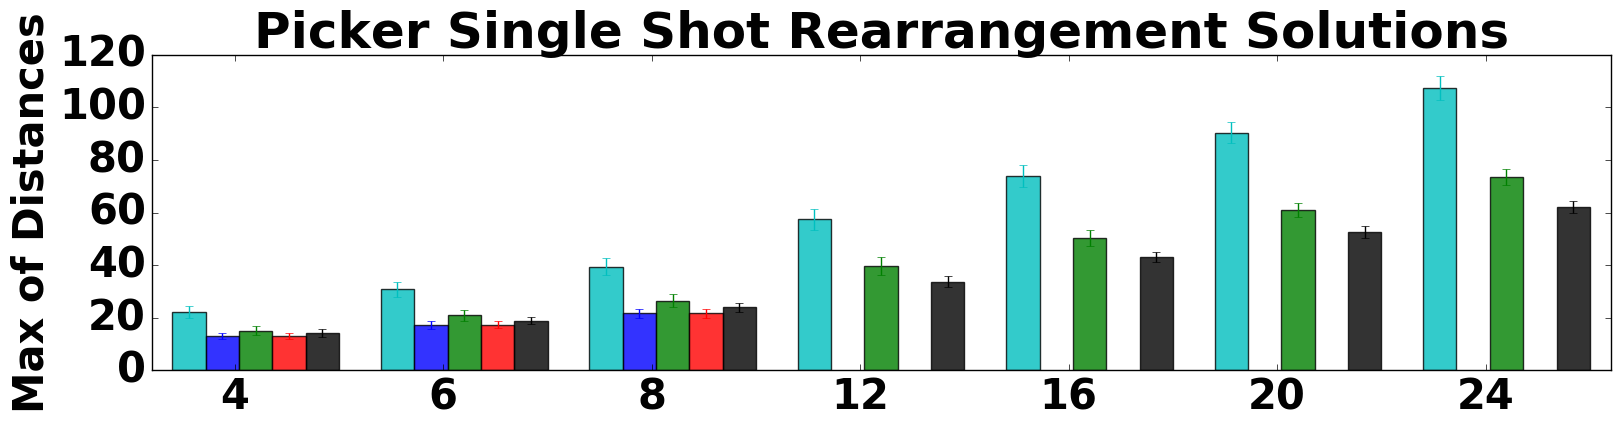
\includegraphics[width=0.48\textwidth]{figures/results/4_sp_ms_cost}
	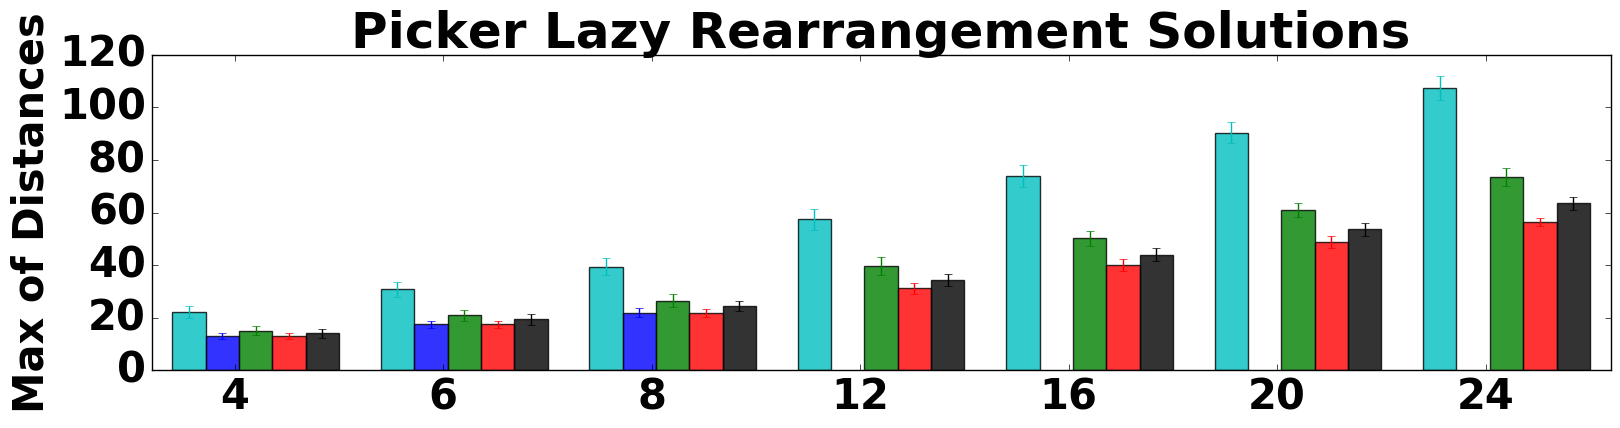
\includegraphics[width=0.48\textwidth]{figures/results/3_sp_lazy_ms_cost}
	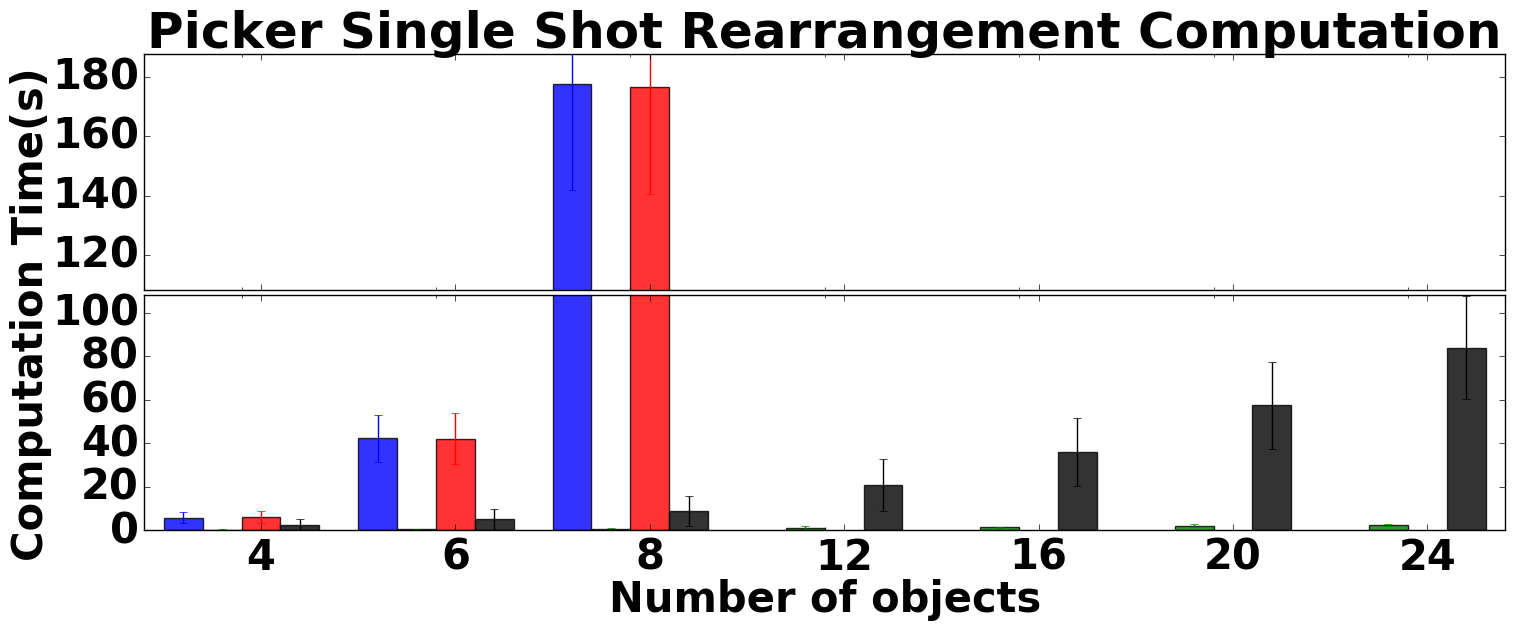
\includegraphics[width=0.48\textwidth]{figures/results/4_sp_ms_time}
	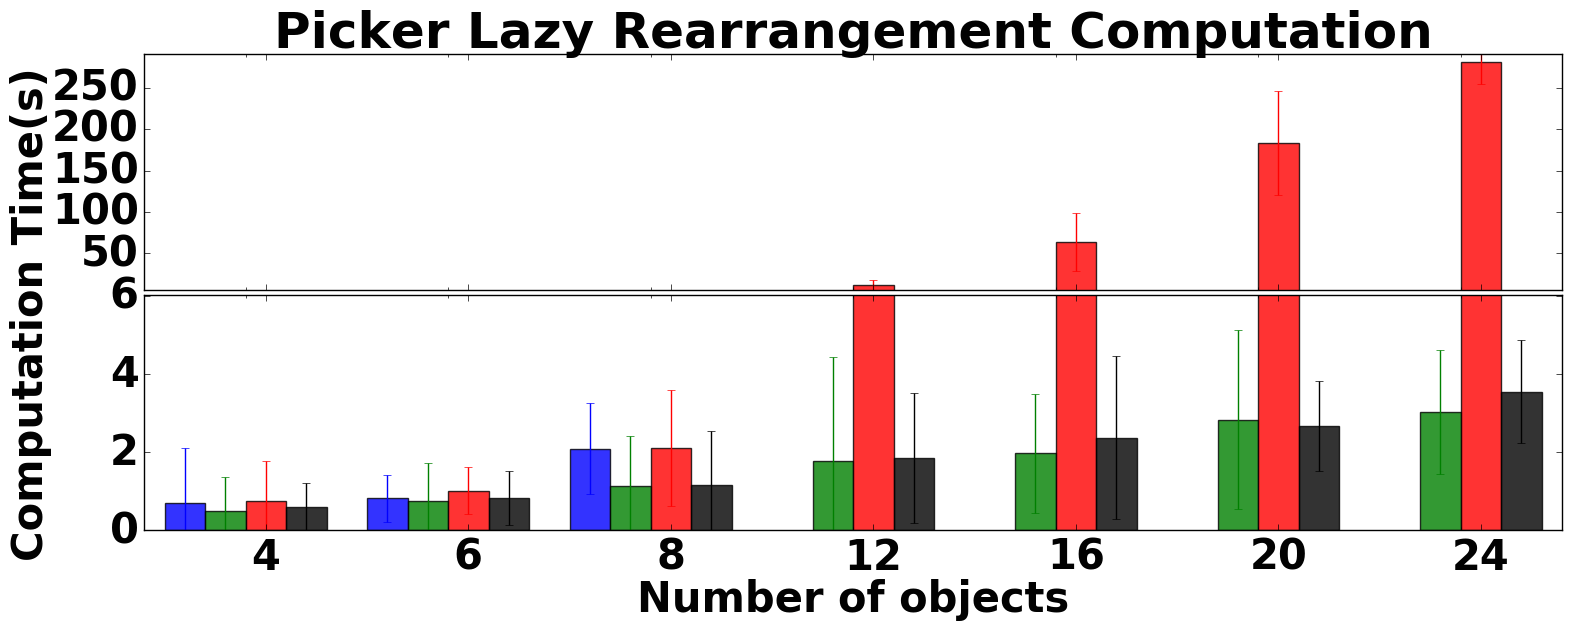
\includegraphics[width=0.48\textwidth]{figures/results/3_sp_lazy_ms_time}
	\vspace{-0.1in}
	\caption{\textit{Simple Picker} results with success\textit{(top)}, solution costs\textit{(middle)}, and computation\textit{(bottom)} reported for single-shot\textit{(left)} and lazy\textit{(right)} versions of the methods}
    \vspace{-0.1in}
	\label{fig:disk}
\end{figure*}

\begin{figure*}[t]
%\vspace{-0.2in}
	\centering
%	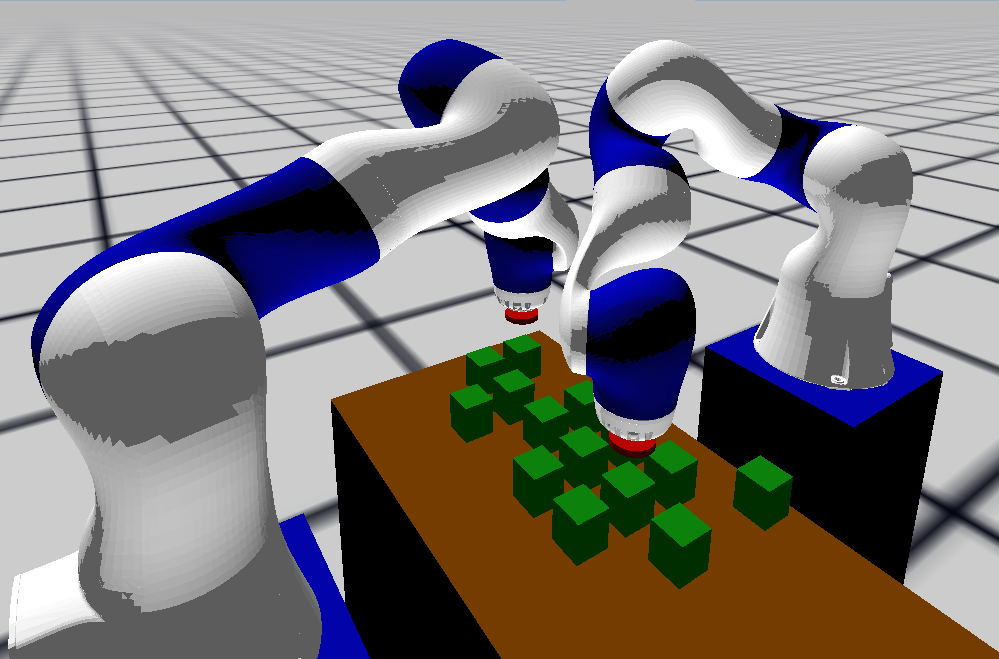
\includegraphics[width=0.48\textwidth]{figures/kuka_benchmark2}
	
\includegraphics[width=0.6\textwidth]{figures/results/labels}
	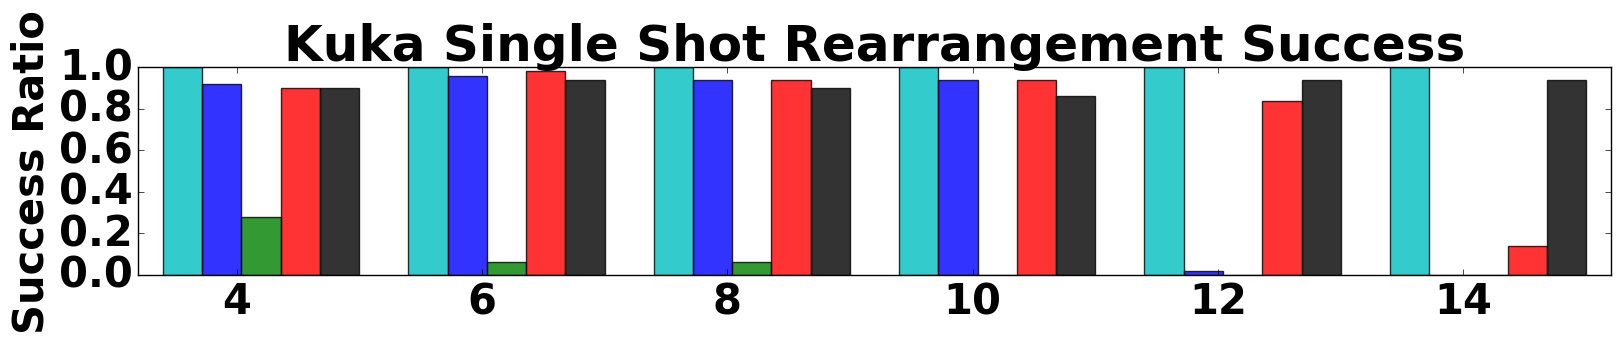
\includegraphics[width=0.48\textwidth]{figures/results/2_kuka_ms_success}
	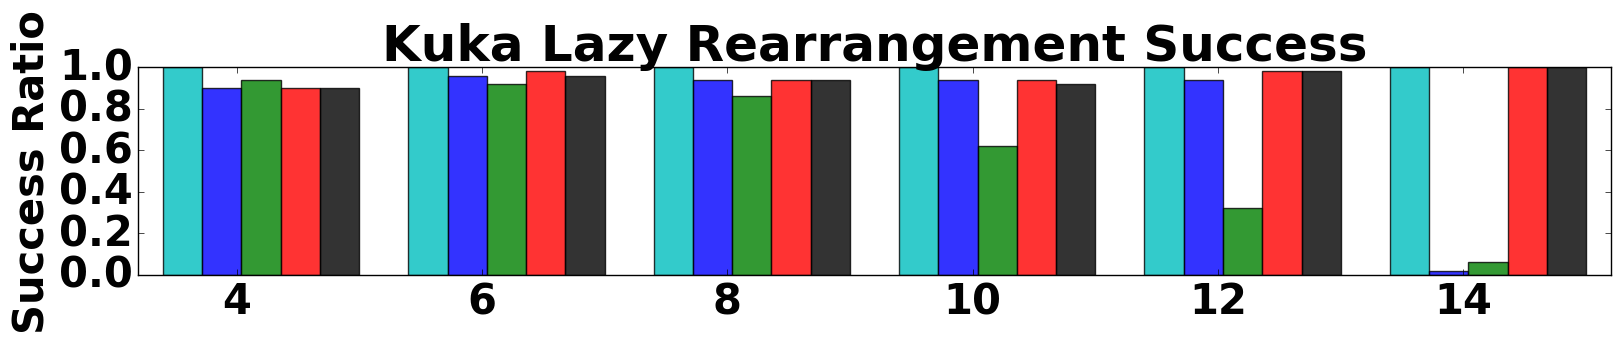
\includegraphics[width=0.48\textwidth]{figures/results/1_kuka_lazy_ms_success}
	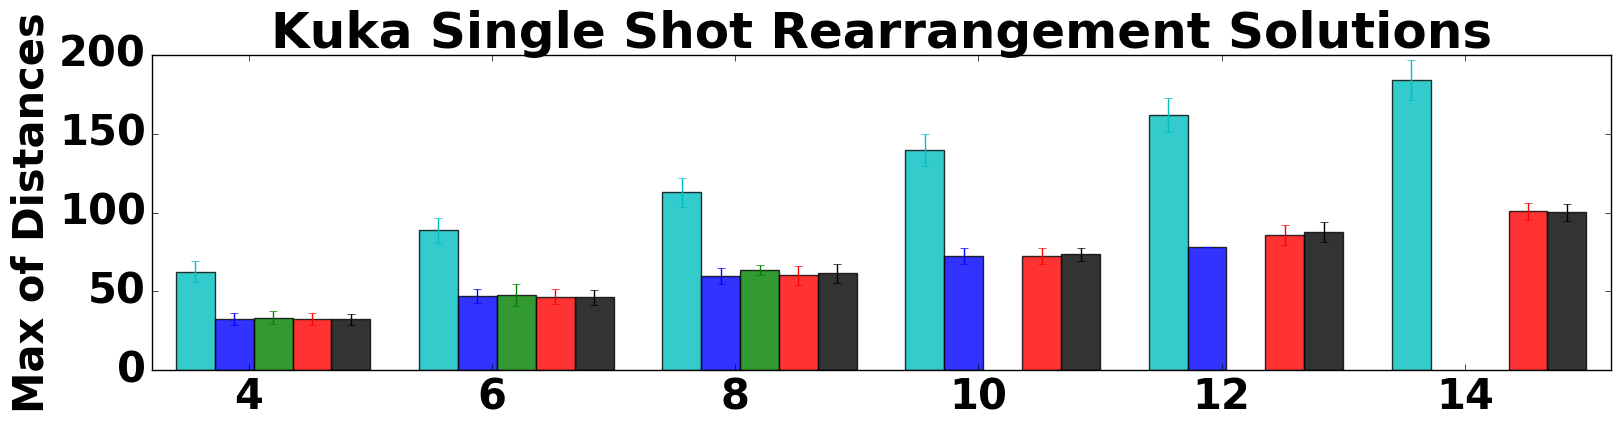
\includegraphics[width=0.48\textwidth]{figures/results/2_kuka_ms_cost}
	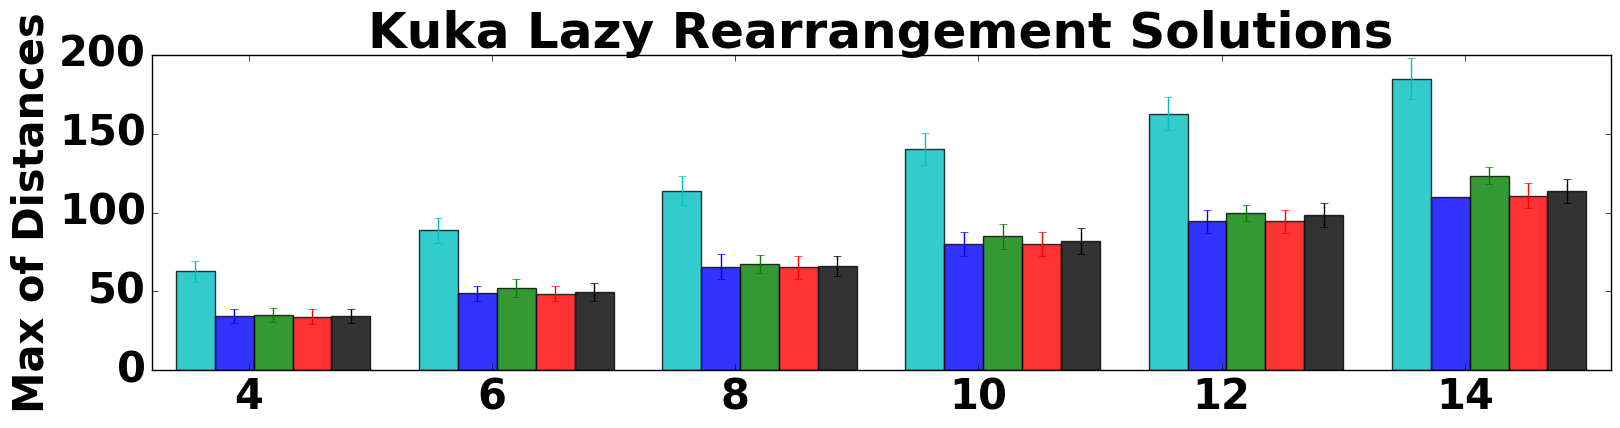
\includegraphics[width=0.48\textwidth]{figures/results/1_kuka_lazy_ms_cost}
	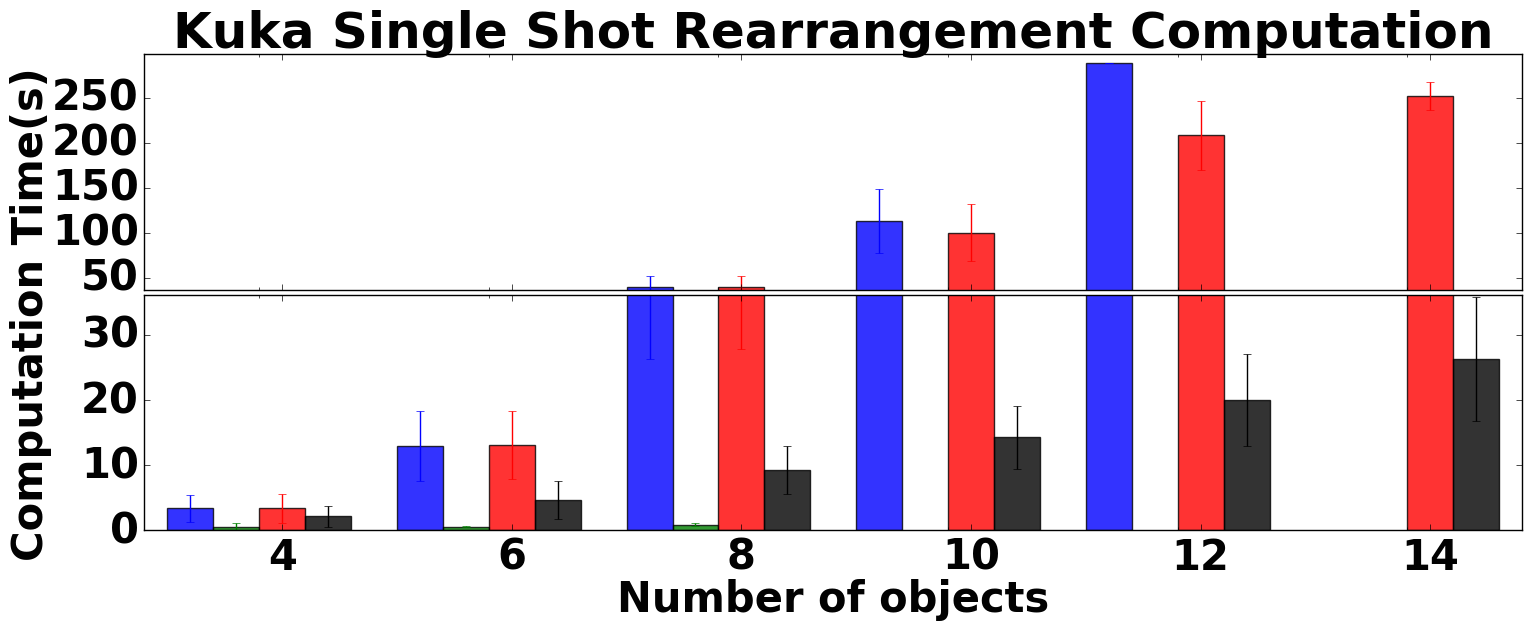
\includegraphics[width=0.48\textwidth]{figures/results/2_kuka_ms_time}
	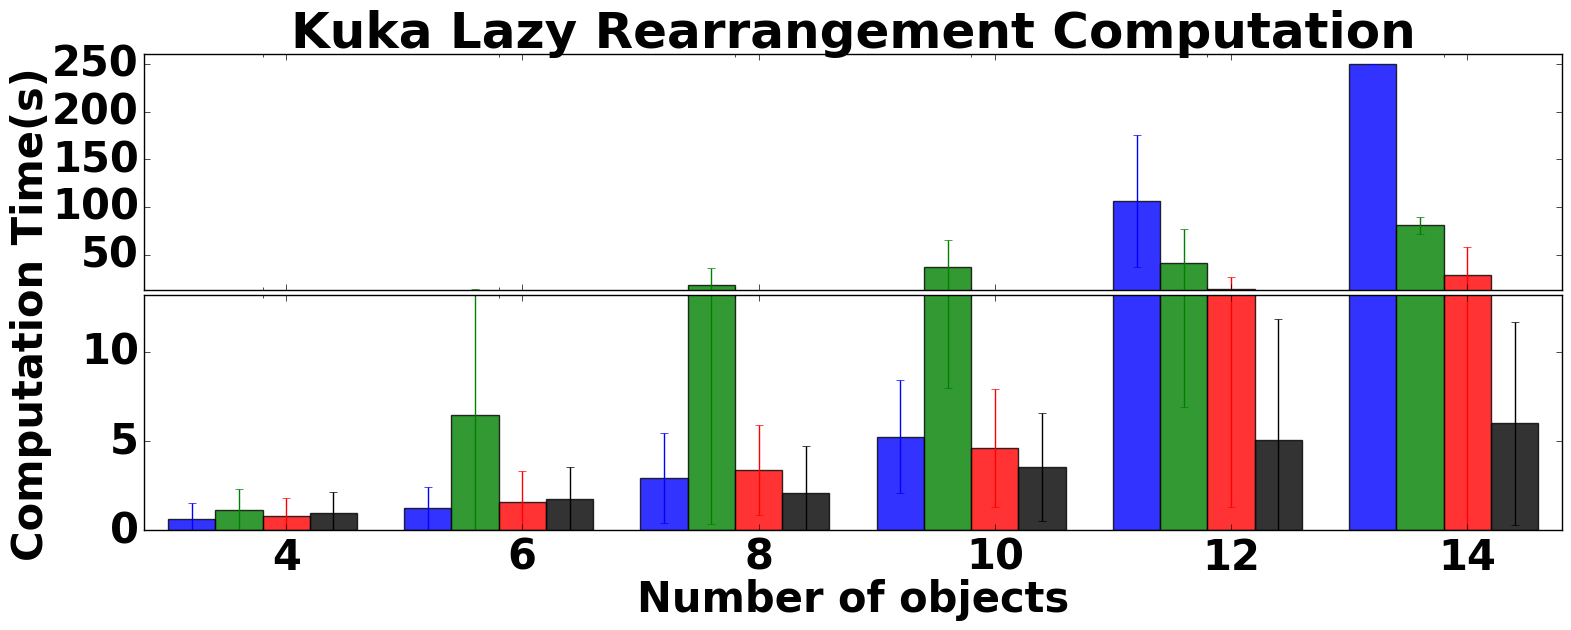
\includegraphics[width=0.48\textwidth]{figures/results/1_kuka_lazy_ms_time}
	\vspace{-0.1in}
    \caption{\textit{\kuka}results with success\textit{(top)}, solution costs\textit{(middle)}, and computation\textit{(bottom)} reported for single-shot\textit{(left)} and lazy\textit{(right)} versions of the methods}
    \vspace{-0.2in}
	\label{fig:kuka}
\end{figure*}




This section describes the experiments performed to evaluate the algorithms in two  domains shown in Fig~\ref{fig:benchmarks}: a) simple picker and b) general manipulators.
%\begin{figure}[ht]
%	\centering
%	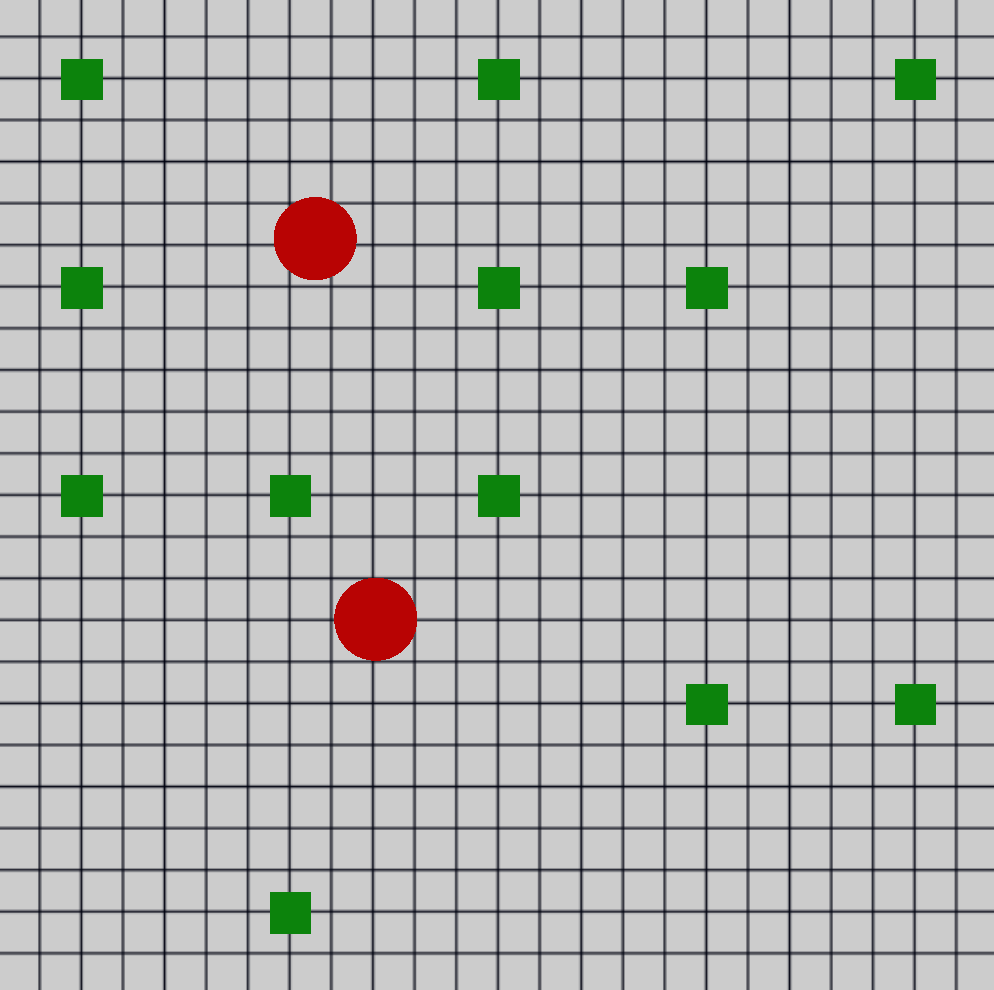
\includegraphics[width=1.9in]{figures/simple_picker_benchmark}
%	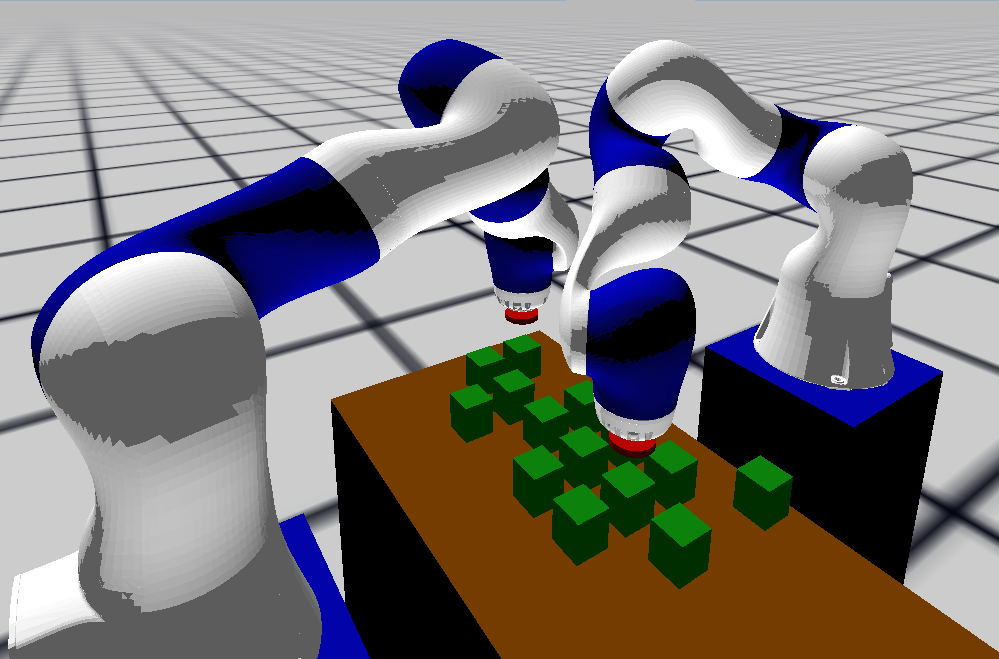
\includegraphics[width=1.8in]{figures/kuka_benchmark2}
%	\caption{The benchmarks: \textit{Simple Picker} and the \textit{General Manipulators} }
%	\label{fig:benchmarks}
%\end{figure}
In order to ensure monotonicity, the object starts and goals do not overlap. Uniform cuboidal objects simplify the grasping problem, though this is not a limitation of the methods. $ 50 $ random experiments were limited to $300s$ of computation time. The underlying $ \drrtstar $ motion planner is restricted to a max of $ 3s $ per plan.
A comparison point includes a random split method, which splits $ \objectset $ at random into two subsets and chooses an arbitrary ordering. Maximum of distances cost is compared to the single arm solution~\cite{193}. Computation times and success rates are reported. The trends in both experiments show that in the single-shot versions, exhaustive and \milp tend to time-out for larger $n$. Lazy variants scale much better for all the algorithms, and in some cases increase the success ratio due to retries. \algo has much better running time than exhaustive and \milp, and produces better and more solutions than random split. Overall, the results show that a) our \milp succeeds more within the time limit than exhaustive, b) \algo scales the best among all the methods, and c) \textbf{the cost of solutions from \algo is close to the optimal baseline}, which is around half of the single arm cost.
% to demonstrate the gains from using multiple arms.  Overall, MILP scales better than exhaustive search, while finding optimal solutions. \algo scales better than the other methods, and finds high quality solutions. The lazy variants improve all the dual-arm methods.

\revisions{Note that we choose to focus on balanced problem instances where at least half of the objects are reachable to one of the robots. Unbalanced instances can be dealt with using {\tt NO\_ACT} object-to-arm assignments that require no dual-arm coordination, while the proposed method remains unchanged.}


\subsection{Simple Picker}
%The results are shown in Figure~\ref{fig:disk}.
This benchmark evaluates two disk robots hovering over a planar surface scattered with objects. The robots are only free to move around in a plane parallel to the resting plane of the objects, and the robots can pick up objects when they are directly above them. This benchmark is reminiscent of delta-robots operating over a picking surface. Fig~\ref{fig:disk}(\textit{top}) all runs up to $ 24 $ objects succeeded for \algo. \milp scales better than exhaustive. Lazy random split succeeds in all cases~(\textit{bottom}). In terms of solution costs~(\textit{middle}) exhaustive finds the true optimal. \milp matches exhaustive and \algo is competitive. In all experiments, \algo enjoys a success rate of 100\% while having much better computation time that exhaustive and \milp, as the number of objects increases. 
% \kiril{What is the reason for low success rate of exhaustive and milp? Is it due to exceeding the time budget?} \kiril{This paragraph misses a statement that demonstrates the benefits of our approach: "In all experiments, \algo enjoys a success rate of \%100, while having much better running time than exhaustive and milp, and producing a higher cost solution than random split. Furthermore, \algo produces a plan whose cost is around half of the single arm plan cost." Similar statements should be added to the other experiments.}

%\subsection{General Manipulator}
%The results are shown in Figure~\ref{fig:kuka}.

\subsection{General Dexterous Manipulator} The second benchmark sets up two \kuka arms across a table with objects on it. The objects are placed in the common reachable part of both arms' workspace, and only one top-down grasping configuration is allowed for each object pose. \revisions{For the Kuka arms top-down reachability exists in an annular region between 40-70cm from the base of each robot. The robots were placed 1.1m apart. Experiments were performed on the largest rectangle that fitted within the intersection of the annular reachability regions.}

Here (Fig~\ref{fig:kuka}) a larger number of motion plans tend to fail, so the single shot variants show artifacts of the randomness of \drrtstar in their success rates. 
% The lazy iterative variants show the robust scalability. 
Random split performs the worst since it is unlikely to chance upon valid motion plans. Single shot exhaustive and \milp scale poorly because of expensive motion planning.
Interestingly, motion planning infeasibility reduces the size of the exhaustive search tree.
The solution costs \textit{(middle)} substantiate benefits of the use of two arms. The computation times \textit{(bottom)} again show the scalability of \algo, even compared to random split.
% In terms of cost. MILP scales to more objects but the computational overhead is more than \algo. Dual-arm solutions are significantly better than single arm.



\tase{
\subsection{Smoothing}
\label{sec:smoothing}


The result of the velocity tuning over the solution trajectories for the individual arms as a post-processing step is shown in Fig~\ref{fig:smoothing}. The objective is to minimize any waits that might be a by-product of the synchronization. 
% The small improvements indicate that synchronization does not adversely affect the solution executions. 
The small \% improvements indicate that the asynchronous variants of the solutions discovered from the methods do not yield a big enough saving in execution time. 
Most of the improvement as a percentage of the original solution duration is not too high. On top of that, the time taken to smooth the solutions for \algo (overlaid on Fig~\ref{fig:smoothing}) shows that the trade-off is sometimes not beneficial.
In their largest problem instances the \kuka spent $ 0.44s $ of smoothing time to save $ 3.23s $ off the solution duration, while the picker spent $  9.84s $ to save $ 0.54s $.

\begin{figure}[t]
	\centering	
	
\includegraphics[width=0.48\textwidth]{figures/results/labels}
	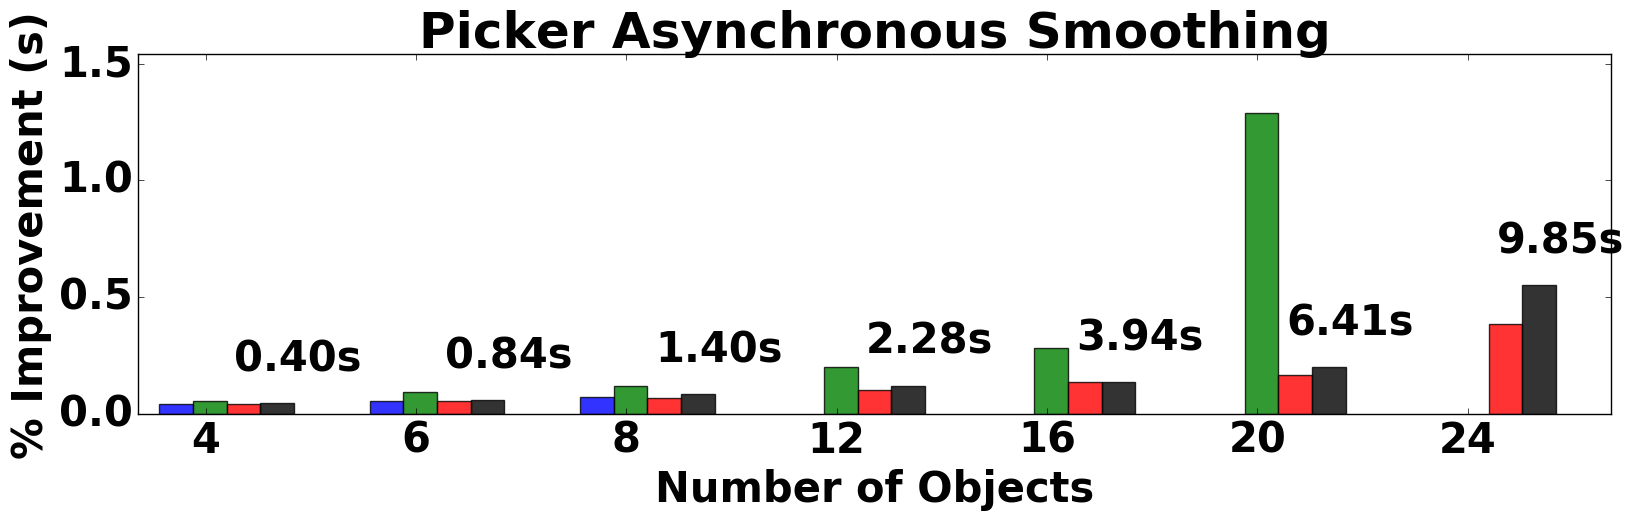
\includegraphics[width=0.48\textwidth]{figures/results/sp_smoothing}
	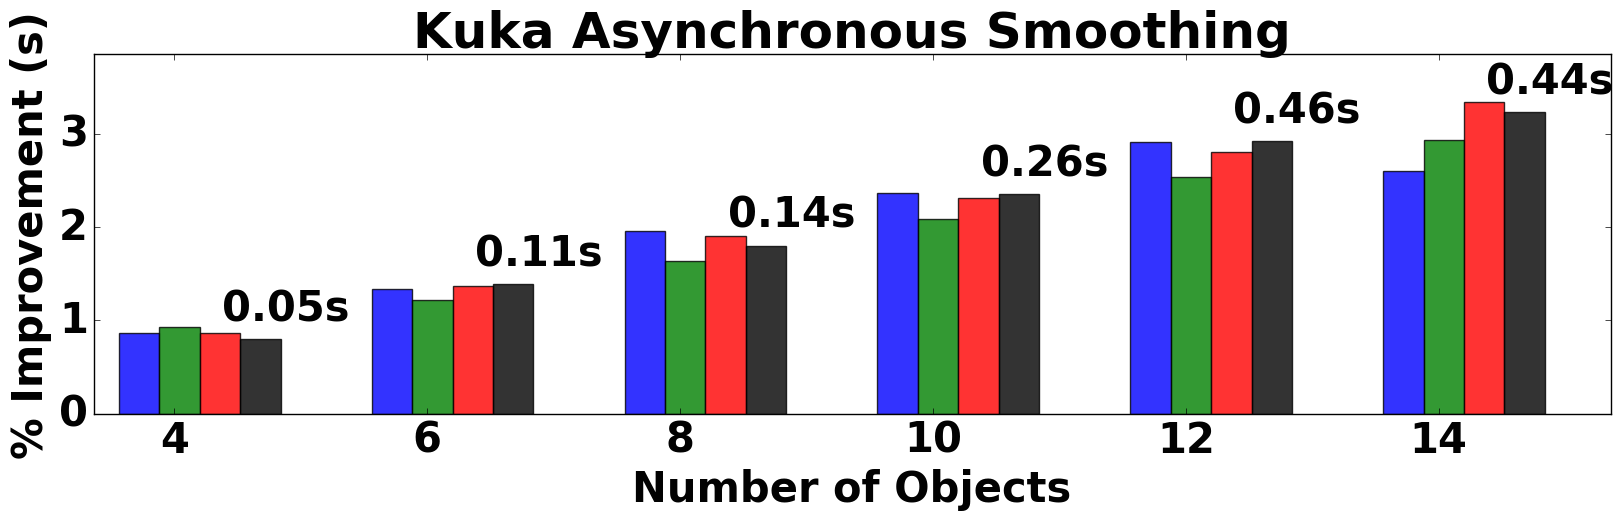
\includegraphics[width=0.48\textwidth]{figures/results/kuka_smoothing}
	\caption{ \tase{Smoothed solution improvement as a percentage of the original synchronized solution duration, and the time taken to smooth solutions obtained from \algo in seconds. } }
	\label{fig:smoothing}
	%     \vspace{-.3in}
\end{figure}

This indicates that among the class of synchronized solutions discovered by the proposed algorithms, the asynchronous, smoothed variants do not seem to be drastically better. Moreover, smoothing does not improve the maximum of distances cost measure, but only reduces the solution duration. 

% The theoretical bounds in the simple planar setups agree with the results in that the synchronization does not degrade the benefits of using 2 arms too much. It should be pointed out though that it needs to be studied further, whether these trends would hold for a class of algorithms that can solve the asynchronous dual-arm rearrangement problem in general setups. This is out of the scope of the current work.

% \kiril{What is the bottom line here? Is smoothing worthwhile? The y-axis in the plots is labeled as \% whereas the bars are labeled with seconds.}

%\clearpage

% \vspace{-0.2in}


\subsection{Reachability Benchmark}
\label{sec:reachability}

In this benchmark, two Kuka arms are placed opposite a target arrangement table, as shown in Fig~\ref{fig:reachability_benchmark}. The initial poses of the objects on either side of the arms in a way that the initial poses are reachable by only one of the arms. The purpose of this study is to see the effects of general divided workspaces where both the initial and target poses are not in the region of common reachability of the arms.  It should be noted that a single arm solution does not exist for this benchmark. 

\begin{figure}[h]
	\centering
	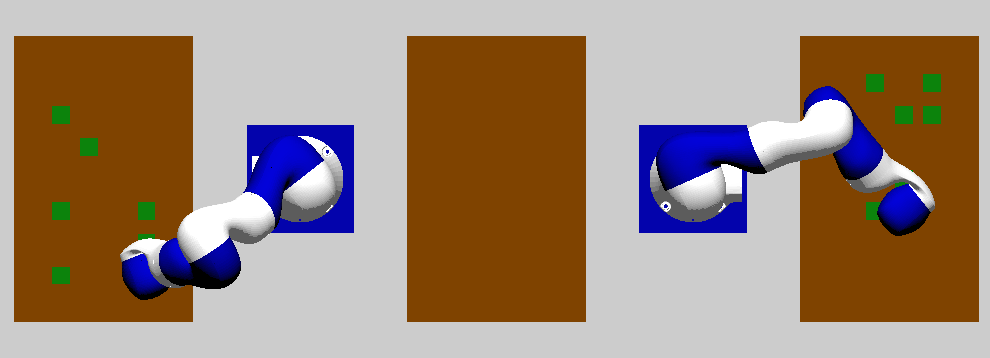
\includegraphics[width=0.48\textwidth]{figures/reachability}
	
\includegraphics[width=0.48\textwidth]{figures/results/labels}
	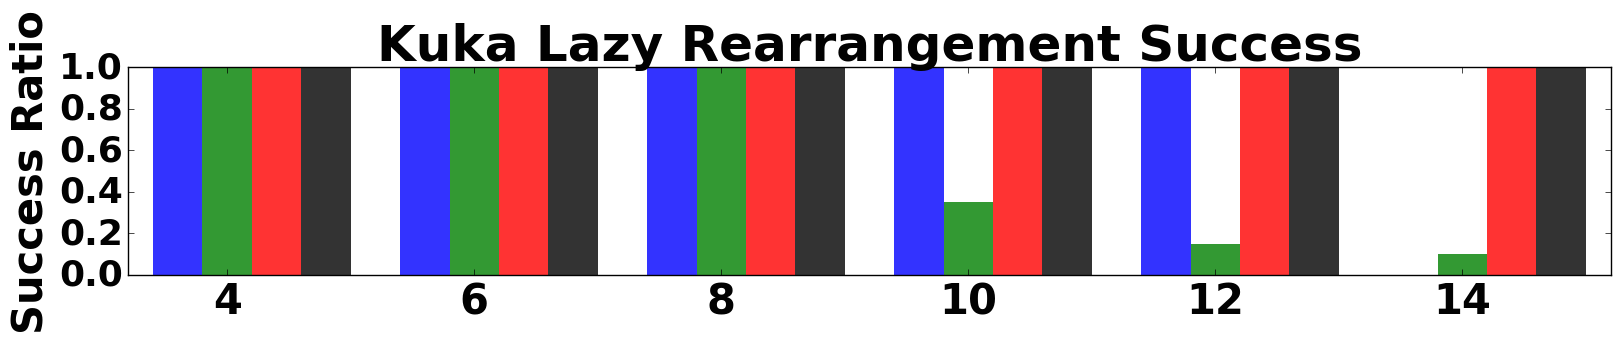
\includegraphics[width=0.48\textwidth]{figures/results/5_kuka_lazy_ms_success.png}
	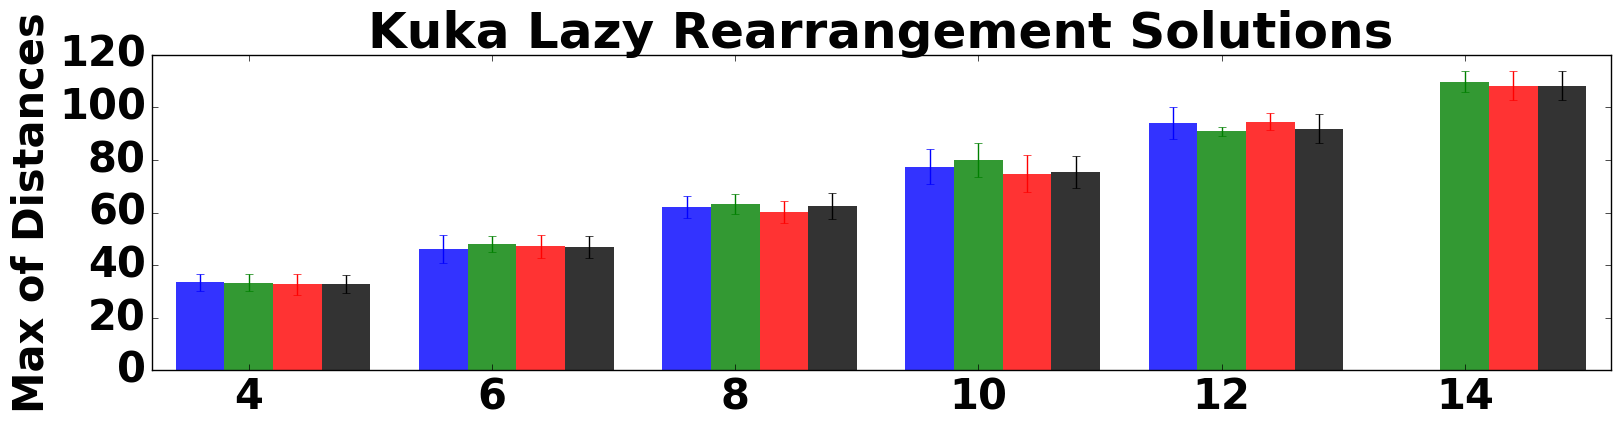
\includegraphics[width=0.48\textwidth]{figures/results/5_kuka_lazy_ms_cost.png}
	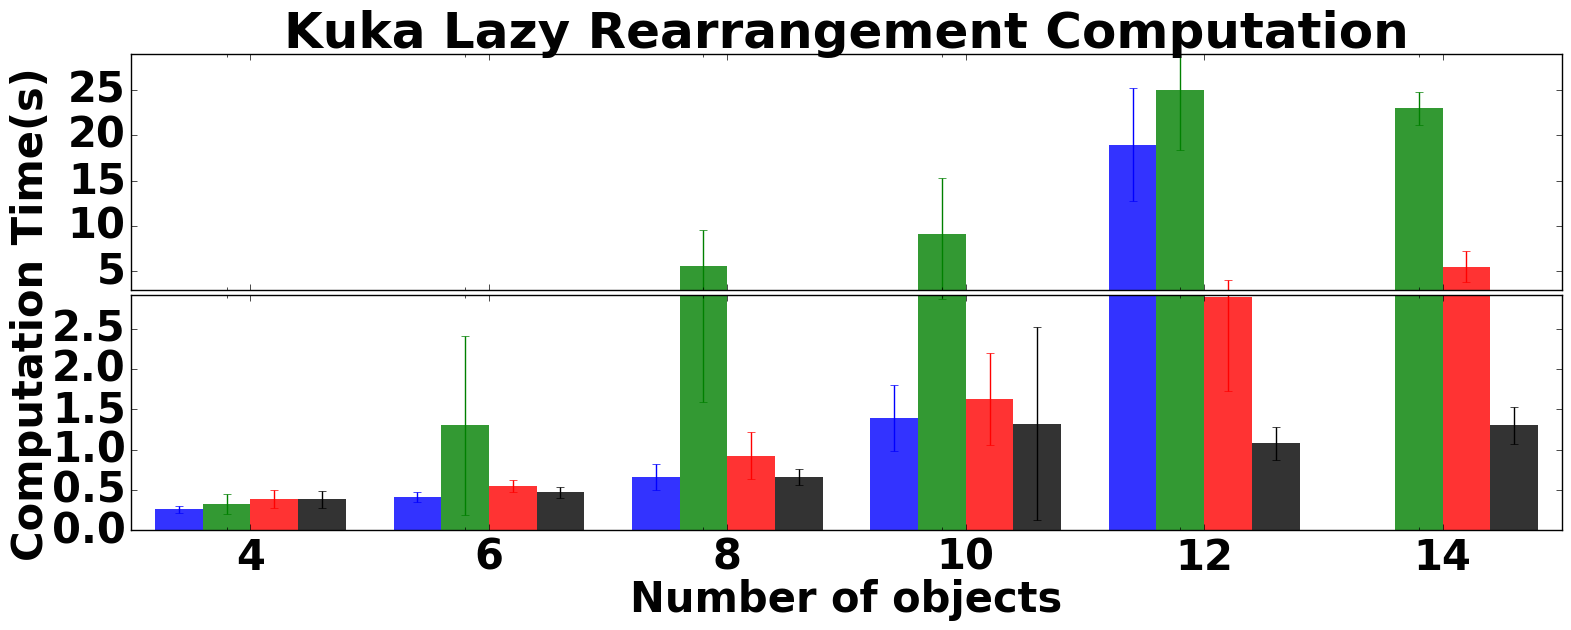
\includegraphics[width=0.48\textwidth]{figures/results/5_kuka_lazy_ms_time.png}
	\caption{ \tase{ The reachability benchmark with the initial poses of the objects lying in disjoint parts of the workspace(tables on the right and left) that are only reachable by one of the arms. The objective is to transfer the objects to the middle table. } }
	\label{fig:reachability_benchmark}
	    \vspace{-.2in}
\end{figure}

The problem of optimizing the assignment of arms to objects will be affected by the reachability. Expectedly, the naive random split tends to erroneously assign unreachable objects to arms. The data reported for the lazy variants, shows that our proposed method manages to maintain scalability and robustness even in such scenarios and moreover, further highlights the benefits of \dual-arm rearrangement.


}

\revisions{\textit{Note on Heuristic Strategies: } 
	%Alternative simplified strategies exist for this problem domain. A significant complexity in the studied problem arises from the coordination of the arms, especially for general manipulators. Decoupled motion planning here with coordination of single-arm solutions is typically faster but loses guarantees of completeness. 
%	For the assignment of objects to arms fast heuristics can be designed to allocate the objects based some partitioning of the workspace. The focus of the current work is however on problems where the arms have to move and coordinate in common regions where such a partition might not exist, and decoupled solutions might not work.
	 It is possible that instead of the random baseline, some other heuristic might be used to allocate the objects to arms, like the proximity of objects to arms or some workspace partitioning. Such a deterministic, decoupled heuristic will make it faster to compute object-arm assignments than the proposed reasoning, but trade off the optimality bounds posited in this work. Given the object-to-arm assignments feasibility of the solution ultimately depends on coordinated motion planning. It should be noted that committing to a single choice of object assignments seriously affects success rates (especially in the Kuka benchmark). The success is only increased using our proposed lazy approach, which takes into account such infeasibility and keeps reattempting other alternatives. A deterministic heuristic however will not offer alternative object-arm assignments and thus is incompatible with the improvements obtained from lazy evaluation. As such we leave the learning and incorporation of appropriate heuristics in this domain as future work and a motivation for practitioners.}

